\documentclass[a4paper,12pt]{article}
\usepackage{amssymb,amsfonts,amsmath}
\usepackage[english]{babel}
\usepackage{latexsym}
\usepackage{tikz}
\usetikzlibrary{decorations.pathreplacing}
\usepackage{epsfig}

% =======================================================================
% Margins --- save forests
\NeedsTeXFormat{LaTeX2e}
\oddsidemargin -10 pt       %   Left margin on odd-numbered pages.
\evensidemargin 10 pt       %   Left margin on even-numbered pages.
\marginparwidth 1 in        %   Width of marginal notes.
\oddsidemargin -1.5 true cm %   Note that \oddsidemargin = \evensidemargin
\evensidemargin -1.5 true cm
\marginparwidth 0.75 in
\textwidth 7.5 true in % Width of text line.
\textheight 26.0 true cm
\topmargin -2.5 true cm

% =======================================================================
% Environments problem, solution, remark

\newcount\probcnt
\newenvironment{problem}[1]{%
  \global\advance\probcnt1%
  \goodbreak\medskip\par\noindent\textbf{Problem~\the\probcnt%
    \if\relax\detokenize{#1}\relax\else~(#1)\fi.}~}%
{%
  \goodbreak
}

\newenvironment{solution}[1][]{%
  \goodbreak\smallskip\par\noindent\textbf{Solution\if\relax\detokenize{#1}\relax\else~#1\fi.}~}%
{%
  \goodbreak
}

\newenvironment{remark}[1][]{
  \goodbreak\smallskip\par
  \small
  \noindent\textbf{Remark\if\relax\detokenize{#1}\relax\else~#1\fi.}~%
}{%
  \goodbreak
  \normalsize
}

\newenvironment{lemma}[1][]{
  \goodbreak\smallskip\par
  \noindent\textit{Lemma\if\relax\detokenize{#1}\relax\else~#1\fi.}~%
}{%
  \goodbreak\smallskip
}

\newenvironment{proof}[1][]{
  \goodbreak\par
  \noindent\textit{Proof\if\relax\detokenize{#1}\relax\else~#1\fi.}~%
}{%
  \goodbreak\smallskip
}


% =======================================================================
%%% Some common macros
\newcommand{\RR}{{\mathbb{R}}}
\newcommand{\ZZ}{{\mathbb{Z}}}
\newcommand{\CC}{{\mathbb{C}}}
\newcommand{\QQ}{{\mathbb{Q}}}
\newcommand{\NN}{{\mathbb{N}}}
\newcommand{\tr}{\rm tr}
\newcommand{\ds}{\displaystyle}
\newcommand{\dx}{\mathrm{d}x}
\newcommand{\dy}{\mathrm{d}y}
\newcommand{\dz}{\mathrm{d}z}
\newcommand{\dt}{\mathrm{d}t}
\newcommand{\du}{\mathrm{d}u}
\newcommand{\GL}{\operatorname{GL}}
\newcommand{\rk}{\operatorname{rk}}

% == TITLES ==========================================================
\begin{document}
\begin{center}
  {\Large\textbf{Proposed problems for the IMC 2026}}
\end{center}

% =======================================================================
%%% DOCUMENT_BEGIN
% Do not change the document above this point
% =======================================================================

% =======================================================================
% My macros
% =======================================================================
% Insert your macros here

% \def\MyMacro{...}


% =======================================================================

\begin{problem}{Alex Avdiushenko, Neapolis University Paphos, Cyprus}
Find all continuous functions
$f: \mathbb{R} \to \mathbb{R}$ with $f(0)=1$ satisfying
\[f(x+y)+f(x-y)=2f(x)f(y) \text{ for all } x,y\in\mathbb{R}.\]

\end{problem}

% -----------------------------------------------------------------------

\begin{solution}
    \\
    \textbf{1. Basic consequences}
    \begin{itemize}
        \item Putting $x=0$ gives $f(y)+f(-y)=2f(0)f(y)=2f(y)$, hence $f$ is even: $f(-y)=f(y)$.
        \item Putting $y=x$ gives $f(2x)=2f(x)^2-1$.
    \end{itemize}

    If $f\equiv 1$, this is a solution. Assume henceforth $f$ is not identically $1$, so there exists $y_0$ with $|f(y_0)|\neq 1$.

    \textbf{2. Construct the companion ``sine-type'' function.}

    Choose $t\in\mathbb{C}$ with $t^2=f(y_0)^2-1$ ($t\neq 0$). Define
    \[h(x) := \frac{f(x+y_0) - f(x-y_0)}{2t}.\]
    Then $h$ is continuous and odd (using the evenness of $f$). Moreover $h(y_0)=t$.

    Moreover, direct computation, using the functional equation twice,
    gives us for all $x,y$
    \[h(x+y) + h(x-y) = 2h(x)f(y). \tag{1}\]
    Swapping $x$ and $y$ and using the oddness of $h$ gives also
    \[h(x+y) - h(x-y) = 2f(x)h(y). \tag{2}\]

    \textbf{3. Factorization of the ``difference''.}

    Define $D(x,y)=f(x+y)-f(x-y)$. A direct manipulation of the given equation shows that for all $x,y,z$,
    \[D(x,y+z)+D(x,y-z) = 2f(z)D(x,y). \tag{3}\]
    In particular, with $z=y_0$ fixed, the function $x\mapsto D(x,y)$ satisfies the linear second order relation
    \[D(x,y+y_0)+D(x,y-y_0)=2f(y_0)D(x,y). \tag{4}\]

    Using the definition of $h$ we have $D(x,y_0)=2t\cdot h(x)$, and $D(0,y)=0$. The function $x\mapsto 2h(x)h(y)$ also satisfies (4) and matches $D(x,y)$ at $x=0$ and $x=y_0$. By uniqueness for this linear relation within continuous functions, it follows that
    \[f(x+y) - f(x-y) = 2h(x)h(y), \text{ for all } x,y. \tag{5}\]

    \textbf{4. Full addition formulas and multiplicativity.}

    Combining the original sum formula with (5), we get the addition formulas:
    \begin{align*}
        f(x+y) &= f(x)f(y) + h(x)h(y),\\
        h(x+y) &= h(x)f(y) + f(x)h(y),
    \end{align*}
    the second coming from adding (1) and (2).

    Define $F(x) := f(x)+h(x)$. Then
    \begin{align*}
        F(x+y) &= f(x+y)+h(x+y)\\
        &= [f(x)f(y)+h(x)h(y)] + [h(x)f(y)+f(x)h(y)]\\
        &= [f(x)+h(x)][f(y)+h(y)]\\
        &= F(x)F(y).
    \end{align*}
    Moreover $F$ is continuous and $F(0)=1$. Hence there exists $c\in\mathbb{C}$ such that
    \[F(x) = e^{cx} \text{ for all } x.\]

    Since $h$ is odd, $f$ is the even part of $F$:
    \[f(x) = \frac{F(x)+F(-x)}{2} = \frac{e^{cx}+e^{-cx}}{2} = \cosh(cx).\]

    Because $f$ is real-valued for all real $x$, $c$ must be either real or purely imaginary. Writing $c=a\in\mathbb{R}$ gives $f(x)=\cosh(ax)$; writing $c=ib$ with $b\in\mathbb{R}$ gives $f(x)=\cos(bx)$. The constant solution $f\equiv 1$ corresponds to $a=b=0$.

    These functions indeed satisfy the functional equation and $f(0)=1$.

    \textbf{Final answer.}

    All such functions are exactly:
    \begin{itemize}
        \item $f(x)=\cos(ax)$ for some $a\in\mathbb{R}$, or
        \item $f(x)=\cosh(ax)$ for some $a\in\mathbb{R}$,
    \end{itemize}
    with the constant solution $f\equiv 1$ included as $a=0$.

\end{solution}

% =======================================================================

\begin{problem}{Daniel Volostnov, Neapolis University Paphos, Cyprus}
A deck contains the cards $1,2,\ldots n$. It is split into two stacks.
The first stack is arranged in increasing order, and the second stack is arranged in decreasing order.
Then an alternating shuffle of these two stacks is performed by taking cards from
the first and then from the second.
If one stack runs out, the remaining cards of the other are placed at the end.
How many different final orders of the deck can be obtained?
\\[0.5cm]
\noindent\textit{Example:} $n=6$, the first stack $A=(1,\,3)$, the second $B=(6,\,5,\,4,\,2)$.

\begin{center}
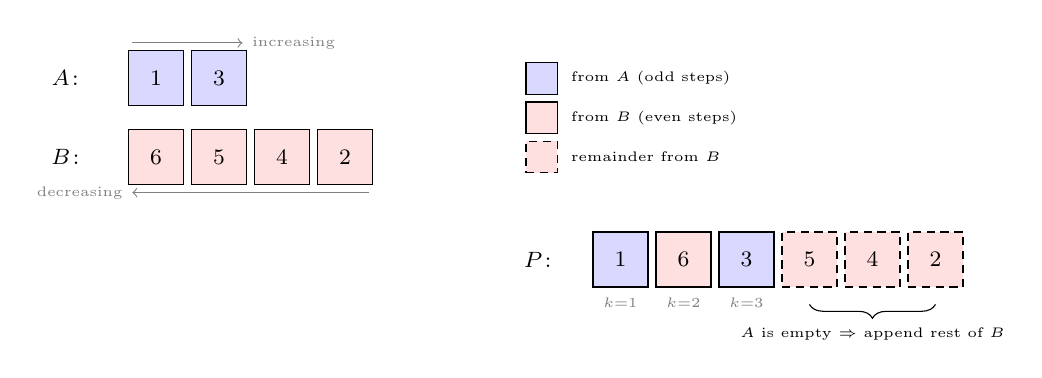
\begin{tikzpicture}[
    box/.style={draw, minimum width=0.7cm, minimum height=0.7cm, inner sep=0pt, font=\footnotesize},
    abox/.style={box, fill=blue!15},
    bbox/.style={box, fill=red!12},
    pbox/.style={box, thick},
    lbl/.style={font=\footnotesize\bfseries},
    arr/.style={->, >=stealth, thick, shorten >=2pt, shorten <=2pt},
    step/.style={font=\scriptsize, fill=white, inner sep=1pt, circle},
    brace/.style={decorate, decoration={brace, amplitude=5pt, raise=2pt}},
  ]

  % --- Deck A ---
  \node[lbl] at (-1.1, 1.8) {$A\colon$};
  \node[abox] (a1) at (0, 1.8) {1};
  \node[abox] (a2) at (0.8, 1.8) {3};

  % --- Deck B ---
  \node[lbl] at (-1.1, 0.8) {$B\colon$};
  \node[bbox] (b1) at (0, 0.8) {6};
  \node[bbox] (b2) at (0.8, 0.8) {5};
  \node[bbox] (b3) at (1.6, 0.8) {4};
  \node[bbox] (b4) at (2.4, 0.8) {2};

  % --- Arrows showing order ---
  \draw[->,gray,thin] (-0.3,2.25) -- (1.1,2.25) node[right,font=\tiny,gray]{increasing};
  \draw[->,gray,thin] (2.7,0.35) -- (-0.3,0.35) node[left,font=\tiny,gray]{decreasing};

  % --- Result P ---
  \node[lbl] at (4.9, -0.5) {$P\colon$};
  \node[pbox, fill=blue!15]  (p1) at (5.9, -0.5) {1};
  \node[pbox, fill=red!12]   (p2) at (6.7, -0.5) {6};
  \node[pbox, fill=blue!15]  (p3) at (7.5, -0.5) {3};
  \node[pbox, fill=red!12, densely dashed] (p4) at (8.3, -0.5) {5};
  \node[pbox, fill=red!12, densely dashed] (p5) at (9.1, -0.5) {4};
  \node[pbox, fill=red!12, densely dashed] (p6) at (9.9, -0.5) {2};

  % --- Step labels under P ---
  \node[font=\tiny,gray] at (5.9,-1.05) {$k{=}1$};
  \node[font=\tiny,gray] at (6.7,-1.05) {$k{=}2$};
  \node[font=\tiny,gray] at (7.5,-1.05) {$k{=}3$};

  % --- Brace for remainder ---
  \draw[brace] (9.9,-1.0) -- (8.3,-1.0)
    node[midway, below=7pt, font=\tiny]{$A$ is empty $\Rightarrow$ append rest of $B$};

  % --- Legend ---
  \node[abox, minimum width=0.4cm, minimum height=0.4cm] at (4.9, 1.8) {};
  \node[font=\tiny, right] at (5.15, 1.8) {from $A$ (odd steps)};
  \node[bbox, minimum width=0.4cm, minimum height=0.4cm] at (4.9, 1.3) {};
  \node[font=\tiny, right] at (5.15, 1.3) {from $B$ (even steps)};
  \node[box, densely dashed, fill=red!12, minimum width=0.4cm, minimum height=0.4cm] at (4.9, 0.8) {};
  \node[font=\tiny, right] at (5.15, 0.8) {remainder from $B$};

\end{tikzpicture}
\end{center}
\end{problem}

% -----------------------------------------------------------------------

\begin{solution}

\textbf{Setup.}
Define the \emph{reference string} $\mathcal{S} = ABAB\cdots$ of length~$n$.
For a given subset~$Y$ of cards in the first stack, let $\mathcal{S}_P \in \{A,B\}^n$ be the \emph{source string} of $P(Y)$: $(\mathcal{S}_P)_i = A$ if the card at position~$i$ of~$P$ came from deck~$A$, and $(\mathcal{S}_P)_i = B$ otherwise.

For $i \in \{1,2,\ldots,n\}$, define
\[
  B_i = \bigl\{\,P(Y) \;\big|\; \text{the smallest index } j \text{ with } (\mathcal{S}_P)_j \neq \mathcal{S}_j \text{ equals } i \bigr\},
\]
and let $B_{n+1} = \bigl\{\,P(Y) \;\big|\; \mathcal{S}_P = \mathcal{S}\bigr\}$ (i.e.\ the source string matches the reference string perfectly).

For each~$i$, let $G_i$ be the directed graph on vertex set $\{1,2,\ldots,n\}$ where there is an edge from $x$ to $y$ whenever $P_x > P_y$, encoding the relative-order structure common to all orders of~$B_i$.

Throughout, assume $i < j$.

\medskip
\textbf{Step 1.} \textit{$B_i \cap B_j = \varnothing$ whenever $j - i$ is odd.}

Consider the graphs $G_i$ and $G_j$, and look at vertices $n-1$ and $n$. For $i$ and $j$ of different parity, the edge between $n-1$ and $n$ is directed in opposite ways in $G_i$ and $G_j$. If a common order existed in $B_i \cap B_j$, it would simultaneously require $P_{n-1} > P_n$ and $P_{n-1} < P_n$, a contradiction.

\medskip
\textbf{Step 2.} \textit{$B_i \cap B_j = \varnothing$ whenever $j - i$ is even and $j - i > 2$.}

Consider the graphs $G_i$ and $G_j$ at vertices $i$ and $i+2$. By the same argument as in Step~1, the edges between these vertices point in opposite directions, giving a contradiction.

\medskip
\textbf{Step 3.} \textit{$B_{n+1}$ creates a single exceptional overlap with $B_n$.}

The set $B_{n+1}$ is on equal footing with the other $B_i$: Steps~1 and~2 apply to it as well, so $B_{n+1}$ is disjoint from all $B_i$ except possibly $B_{n-1}$ and $B_n$ (by parity).
In fact, $B_{n+1}$ and $B_n$ share exactly one order: the sequence $P = (1, n, 2, n{-}1, \ldots)$ produced by $A = \{1, 2, \ldots, \lceil n/2 \rceil\}$ and $B = \{n, n{-}1, \ldots, \lfloor n/2 \rfloor + 1\}$.
This is because the edge $n{-}1 \to n$ does not appear in $G_{n+1}$, so the graph constraint of $G_n$ is also satisfied. No other order of $B_{n+1}$ lies in~$B_n$.

\medskip
From Steps 1--3 it follows that $B_1 \cup B_2 \cup \cdots \cup B_{n+1} = \{P(Y) : Y \subseteq S\}$, and the only non-empty pairwise intersections are $D_i := B_i \cap B_{i+2}$ for $i = 1, \ldots, n-1$, together with the single exceptional order $|B_n \cap B_{n+1}| = 1$.

\medskip
\textbf{Step 4.} \textit{Computing $|B_i|$.}

The graph $G_i$ consists of two directed paths (``bamboo sticks''). Since each $B_i$ encodes all possible subsets $Y$ whose source string first deviates from $\mathcal{S}$ at position~$i$, the bamboo lengths depend on the parity of~$i$:
\begin{itemize}
  \item if $i$ is odd: $|B_i| = \displaystyle\binom{n}{(i-1)/2}$,
  \item if $i$ is even: $|B_i| = \displaystyle\binom{n}{n - i/2 + 1}$.
\end{itemize}
Since all $B_i$ together (for $i = 1, \ldots, n+1$) partition the set of source-string encodings of all $2^n$ subsets, we have
\[
  \sum_{i=1}^{n+1} |B_i| = 2^n.
\]

\medskip
\textbf{Step 5.} \textit{Computing the overlaps $|D_i|$ where $D_i = B_i \cap B_{i+2}$.}

From Steps 1 and 2, $D_i \cap D_j = \varnothing$ for $i \neq j$. Consider the union graph $G'$ of $G_i$ and $G_{i+2}$. For odd~$i$, the graph $G'$ is almost identical to $G_{i+2}$ except that edges $i \to i+1$ and $i+1 \to i+2$ are added, which fix the relative order of $(i+1)/2$ vertices. Removing these determined vertices leaves two bamboo sticks, one with $(i-1)/2$ vertices. Hence for odd $i$,
\[
  |D_i| = \binom{n - (i+1)/2}{(i-1)/2}.
\]
Substituting $i = 2h + 1$ gives $|D_i| = \binom{n - 1 - h}{h}$.

An analogous argument for even $i = 2h + 2$ yields $|D_i| = \binom{n - 2 - h}{h}$.

\medskip
\textbf{Step 6.} \textit{Assembling the answer.}

By inclusion--exclusion,
\[
  N(n) = \sum_{i=1}^{n+1} |B_i| - 1 - \sum_{i=1}^{n-1} |D_i|,
\]
where $-1$ accounts for the single exceptional overlap $|B_n \cap B_{n+1}| = 1$ from Step~3.

The sum of $|B_i|$ equals $2^n$ (Step~4).

The sum over odd-indexed $D_i$ ($i = 1, 3, 5, \ldots$): when $n$ is odd this equals $F_n - 1$; when $n$ is even this equals $F_n$. Similarly, the sum over even-indexed $D_i$ ($i = 2, 4, 6, \ldots$): when $n$ is odd this equals $F_{n-1}$; when $n$ is even this equals $F_{n-1} - 1$.

In both cases the total is
\[
  \sum_{i=1}^{n-1} |D_i| = F_n + F_{n-1} - 1 = F_{n+1} - 1.
\]

Therefore,
\[
  \boxed{N(n) = 2^n - 1 - (F_{n+1} - 1) = 2^n - F_{n+1}},
\]
where $F_{n+1} = F_n + F_{n-1}$ is the $(n{+}1)$-th Fibonacci number (with $F_1 = F_2 = 1$).

\medskip
\textbf{Grading guidelines} (scores do not accumulate):
\begin{itemize}
  \item 2 points --- a correct recurrence formula for $N(n)$;
  \item 3 points --- a correct closed-form formula;
  \item 5 points --- correct formula with a recursive/structural proof that has a significant gap;
  \item 7 points --- correct formula with a minor gap that does not materially affect the answer;
  \item 10 points --- complete solution.
\end{itemize}

\smallskip
\begin{remark}
    \textbf{Note to graders:}
    Recursive/inductive solutions should be scrutinized with particular care.
    Many such arguments sound convincing at first glance but break down
    upon closer inspection of boundary cases and transitions to known identities.
\end{remark}

\end{solution}

% =======================================================================
% Do not change the document below this point
%%% DOCUMENT_END
% =======================================================================

\end{document}

